\section{Theory}
\textcolor{magenta}{\textbf{This is work in progress. Align with previous chapters when they are written}}


\begin{comment}
\textcolor{magenta}{\textbf{What must be clear by now
	 \begin{itemize}
	 	\item Consider case without covariates
	 	\item Make clear that SC is a weighted average of the donors
	 \end{itemize}}}
\end{comment}
In this chapter, we propose an alternative \ac{SC}-estimator to assess the magnitude of treatment effects in observational settings. To establish a general basis, let us first describe the contextual environment of the estimation. Similar to the setting as introduced by \ac{ADH}, we consider a framework with $J+1$ panel units indexed by $j = 0,1, ..., J$ that are observed over a time horizon of $T$ periods. Without loss of generality, assume that unit $j = 0$, is exposed to the treatment at period $t = T_0$ with $1 < T_0 < T$ and that there are no treatment anticipation and contamination (i.e., no spillovers in time and space). The former would be the case if the treatment affects unit $j = 0$ before $T_0$, the latter describes the case where some of the supposedly untreated units $j = 1,...,T$ are contaminated as they are affected by the treatment. To contextualize these assumptions, \cite{abadie:2010} argue that in the presence of anticipation effects, $T_0$ could be shifted back in time until the assumptions seems plausible. If panel units in the donor pool\footnote{To ensure direct comparability with the \ac{SC} literature, we adopt most of the commonly used terms. For example, control group units are labeled as 'donors'.} are affected by the treatment (contamination) as it is likely in Brexit-application, those units could be removed from the sample prior to the estimation. Our goal is to evaluate the causal effect of the treatment, the specific functional form of which remains unspecified though. This is possible because the main goal of the \ac{SC}-estimation lies in the precise estimation of the counterfactual. Since the treatment  scenario is empirically observable, it is not necessary to specify the functional form of it (e.g. level or slope shift, fading or persistent shock).

The following theoretical argumentation is structured as follows: We first describe the canonical estimation procedure as proposed by \ac{ADH}. Next we build intuition by considering a simple static scenario with only two donor units and one treatment unit that is then generalized to the case with many donors. The main difference between our extensions and the setting of \ac{ADH} is that we remove some of the weight constraints and that we analyze a situation without covariates. The former distinction guides us to the field of regularization in order to prevent our method from overfitting. The latter drastically reduces the data requirements but causes our algorithm to estimate the counterfactual with a significantly smaller information set. This fact leads us to our main contribution: The integration of  multivariate time series approaches into the \ac{SC}-algorithm. 

\subsection{ADH Case}
We start by presenting the \ac{SC}-method in its original form as introduced \ac{ADH}. Besides introducing the general estimation technique, we also want to elaborate on the proposed hypothesis testing procedure of \ac{ADH}. For the sake of comparability and due to its notational and inhat clarity, we borrow the employed notation of Abadie and colleagues. In terms of the structural design, we build on the thorough presentation of \ac{SC} and the proposed hypothesis testing procedure by \cite{firpo:2018}.

\textit{Setup} \\
The estimation task can be constituted by the potential outcome framework as introduced by \cite{neyman:1923} and elaborated by \cite{rubin:1974}. Let $Y^{I}_{j,t}$ be the (potential) outcome for unit $j$ at point $t$ in the presence of the intervention. Likewise, let $Y^{N}_{j,t}$ be the (potential) outcome for $j$ at point $t$ in the absence of the intervention. \ac{ADH} define the treatment effect of the intervention as 
\[
\delta_{j,t} = Y^{I}_{j,t} - Y^{N}_{j,t}
\] 
and introduce the indicator variable $D_{j,t}$ that takes on the value 1 if unit $j$ is treated at period $t$ and the value 0 otherwise. Given the assumed absence of anticipation and contamination, we observe the following outcome
\[
Y_{j,t} + D_{j,t} \delta_{j,t} = 
\begin{cases}
	Y^{N}_{j,t} &\text{(if } j = 0 \text{ and } t < T_0\text{)} \text{ or } j \geq 1, \\
	Y^{N}_{j,t} + \delta_{j,t} &  \text{\phantom{(}if } j = 0 \text{ and } t \geq T_0
\end{cases}
\] 
The goal to estimate the causal treatment effect $(\delta_{0,T_0}, ..., \delta_{0,T})$ therefore boils down to the estimation of the counterfactuals of unit $j = 0$ in the post-treatment phase $(Y_{0,T_0}, ..., Y_{0,T})$, i.e. on what trajectory would unit $j=0$ have beeen had there been no intervention. The basic idea of \ac{ADH} is to estimate these counterfactuals as a weighted average of the donor outcomes, using a data-driven approach to compute the weights. Intuitively, the weights are computed such that they optimally predict the outcomes and a set of explanatory variables of the treatment unit in the pre-intervention phase, conditional on having a percentage interpretation. To operationalize this intuition, let $\boldsymbol{Y_j} = (Y_{j,1}, ..., Y_{j,T_0})^\prime$ be the vector of observed outcomes in the pre-treatment phase for unit $j$\footnote{For instance, in the canonical example of \cite{abadie:2003}, $\boldsymbol{Y_j}$ would be the vector of \ac{GDP}s for panel unit $j$.}. To distinguish treatment unit and donors, \ac{ADH} denote the $(T_0 \times 1)$-vector of the treatment unit as $\boldsymbol{Y_1}$ and the $(T_0 \times J)$-matrix of the donors as $\boldsymbol{Y_0}$. Moreover, a set of $K$ covariates is observed for all panel units for $t = 1,2,...,T$, yet only the pre-treatment values are needed for the weight-calculation. Therefore, let $\boldsymbol{X_1}$ denote the $(K \times 1)$-vector of covariates for $\boldsymbol{Y_1}$ and let $\boldsymbol{X_0}$ denote the $(K \times J)$-matrix of explanatory variables for $\boldsymbol{Y_0}$. In order to estimate the causal effect of the treatment, the \ac{SC}-estimator estimates the counterfactuals $(\widehat{Y}_{0,1}, ...,\widehat{Y}_{0,T_0},..., \widehat{Y}_{0,T})$ for the pre- and post-intervation phase as 
\[
\widehat{\boldsymbol{Y}}^{N}_{0,t} = \sum_{j = 1}^{J} \widehat{w}_j Y^{N}_{j,t} \text{ } \forall \text{ } t \in \{1,...,T\}
\]
The weights are stacked in the vector $\boldsymbol{\widehat{W}} = (\widehat{w}_1, ... , \widehat{w}_J)^\prime$ and have the constraint to have a percentage interpretation such that $\widehat{w_j} \geq 0$ and $\sum_{j = 1}^{J} \widehat{w_j} = 1$. It is worth noting that the percentage interpretation of the weights requires the counterfactuals to belong to the convex hull of the donors as otherwise, $\widehat{\boldsymbol{Y}}^{N}_{0,t}$ will never match its true counterpart. \cite{abadie:2010} argue that "the magnitude of discrepancy" should be calculated in advance of each \ac{SC}-application. If the researcher finds that the pre-intervention values of $\widehat{\boldsymbol{Y}}^{N}_{0,t}$ fall outside the convex hull of the donors, the employment of \ac{SC} is not recommended. The weights $\boldsymbol{\widehat{W}}$ are obtained as the solution of a nested optimization problem that aims to match both the pre-treatment outcomes ($\boldsymbol{Y_1}$) and a set of fixed pre-treatment covariates for the treatment unit ($\boldsymbol{X_1}$). \ac{ADH} formalize this idea as follows
\[
\widehat{\boldsymbol{W}}(\boldsymbol{V}) = 
\underset{\text{s. t. }\widehat{w_j} \geq 0 \text{ and } \sum_{j = 1}^{J} \widehat{w_j} = 1}{\arg\min}
(\boldsymbol{X_1} - \boldsymbol{X_0}\boldsymbol{W})^\prime \boldsymbol{V}(\boldsymbol{X_1} - \boldsymbol{X_0}\boldsymbol{W})
\]
with $\boldsymbol{V}$ being an arbitrary diagonal positive semidefinite weight matrix of dimension $(k \times k)$. $\boldsymbol{V}$ itself is the solution of the following optimization problem
\[
\widehat{\boldsymbol{V}} = 
\underset{\text{s. t. } \widehat{\boldsymbol{V}} \in \mathcal{V}}{\arg\min}
(\boldsymbol{Y_1} - \boldsymbol{Y_0}\boldsymbol{\widehat{W}}(\boldsymbol{V}))^\prime (\boldsymbol{Y_1} - \boldsymbol{Y_0} \boldsymbol{\widehat{W}}(\boldsymbol{V}))
\]
with $\mathcal{V}$ being the set of all positive semidefinite weight matrices of dimension $(k \times k)$. Subsequently, the causal effect of the intervention $\delta_{j,t}$ can be quantified at each time point after the intervention $t = t_0 +1, ..., T$ as the gap between observed ($Y^{N}_{0,t} + \delta_{j,t}$) and predicted outcome ($\widehat{Y}^{N}_{0,t}$).

This two-step estimation procedure serves two crucial purposes: $\widehat{\boldsymbol{V}}$ measures the relative importance of the variables in $\boldsymbol{X_0}$ to explain $\boldsymbol{X_1}$. Specifically, $\widehat{\boldsymbol{V}}$ is selected such that it minimizes the Euclidian distance of the pre-intervention outcome of unit $j = 0$ and its synthesized counterpart defined by $\widehat{\boldsymbol{W}}(\boldsymbol{V})$. The weighting vector $\widehat{\boldsymbol{W}}(\boldsymbol{V})$ in contrast quantifies the relative importance of each unit in the donor pool. Summarizing the key concept of \ac{ADH}, the \ac{SC}-method ensures that the synthesized treatment unit is as similar as possible to the actual treatment unit with respect to the quantity of interest and a set of potential explanatory variables in the pre-treatment period. Especially in the canonical examples of \ac{SC}, the quantity of interest (e.g. \ac{GDP}) and the explanatory variables (e.g. investment, savings etc.) were inherently interconnected. Thus, observing that the \ac{SC}-estimator was capable of approximating both targets significantly enhanced the methods credibility. If explanatory variables are omitted, the \ac{SC}-algorithm reduces to an \ac{OLS} estimation, constraint such that the constant equals zero and that the coefficients have a percentage interpretation.

The main concern when assessing treatment effects with the \ac{SC}-method is the poor 
generalizability of the estimation results in the post-treatment period. For example, especially when employing non-parametric statistical learning methods, it is simple to achieve high in-sample (pre-treatment) fit. The crucial part when dealing with forecasts is that the observed in-sample patterns generalize well outside the verifiable horizon (post-treatment). One way to assess methods for detecting generalizable patterns is through hypothesis testing.

\textit{Hypothesis Testing} \\
\ac{ADH} propose a model-invariant non-parametric inference procedure that is based on the Exact Hypothesis Test proposed by \cite{fisher:1971}. The basic idea behind such permutation tests is to compare the observed data with a number of randomly permuted versions of the data, and to use the distribution of the test statistic calculated from these permuted samples to estimate the probability that the observed result occurred by chance alone. 

In the context of \ac{SC}, \ac{ADH} consider permutations in region (i.e. panel unit) and time. Region permutations estimate the treatment vector $(\delta_{j,T_0}, ..., \delta_{j,T})$ for each panel unit $j \in \{0, ..., J \}$.\footnote{Note that it is necessary to exclude the truly treated unit from donor pool to ensure the validity of the no contamination assumption.} This procedure provides them with the empirical $(J+1)$-observational distribution of the treatment. Subsequently, it is possible to compare the estimated treatment vector $(\delta_{0,T_0}, ..., \delta_{0,T})$ of the treated unit with the $J$ placebo-treatment vectors of the units of the donor pool. Given the estimated treatment effect for $j=0$ is large, the null hypothesis of no treatment effect can be rejected at the significance level of one minus the percentile of $(\delta_{0,T_0}, ..., \delta_{0,T})$ in the empirical distribution.\footnote{For instance, let $J = 99$ such that treatment effects for 100 panel units can be computed. As long as the estimated treatment effect of the truly treated units belongs to the 95 largest effects (95th percentile or higher), the permutation test rejects the null hypothesis of no treatment effect at least at 5 percent.} Time permutations on the other hand consider only panel unit $j = 0$, permute $T_0$ to dates prior to the true treatment date and again compute the empirical treatment distribution. Given that $T_0 > J$, this approach can increase the sensitivity of the test, since the theoretically feasible significance threshold of region permutation tests is determined by $\frac{1}{J}$. For both, region and time permutations, \ac{ADH} condense the vector of estimated treatment effects into a precision metric like the \ac{MSFE}\footnote{Note that \ac{ADH} speak of the Mean Squared Prediction Error for dates before and after $T_0$. Since we consider the time span until $T_0$ as prediction window and the time span after $T_0$ as forecast window, we employ the label \ac{MSPE} before $T_0$ and the label \ac{MSFE} from $T_0$ onward.} of the following form:
\[
MSFE_j = \frac{\sum_{t = T_0}^{T} \left(\widehat{Y_{j,t}^N} - Y_{j,t}^N\right) ^2}{T- T_0}
\]
A potential problem that may arise when examining the relative rarity of the estimated treatment effect using the procedure described above is inherent in the nature of \ac{SC}. In the context of region permutations, suppose that a donor region is very different from the rest such that it falls outside the convex hull of the remaining donors. Note, that this circumstance does not cause problems for the truly treated region and its synthesized counterfactual. The outlier described above is likely to be assigned a weight of zero in the estimation of the potential outcome without treatment. However, since the outlier cannot be synthesized precisely by the donor pool by construction, both \ac{MSPE} and \ac{MSFE} are expected to be large. As this special feature causes the permutation test to be unreasonably conservative, \ac{ADH} propose to exclude regions who are hard to predict, i.e. who have a \ac{MSPE} that exceed the \ac{MSPE} of the truly treated unit to a great extent. 

Figure \ref{F_01} visualizes the exclusion procedure in the tobacco control application of \ac{ADH}. The vertical axis indicates the gap between observed and estimated  per capita cigarette sales, with the bold line representing the truly treated region (California). Looking at panel A, two observations stand out: First of all, the treatment has a clear negative effect for California. Second, some regions have both a poor pre- and post-treatment fit. Since the estimated treatment should not be artificially driven by a poor fit, \ac{ADH} successively remove regions with a large \ac{MSPE} relative to California. Panel B excludes regions with a \ac{MSPE} that is more than 20 times as large the \ac{MSPE} of California, Panel C lowers the cutoff to five times California's \ac{MSPE} and Panel D to  two times the \ac{MSPE}. In the last scenario, only 19 regions are left and California is the one with the most extreme treatment effect. The treatment is therefore statistically significant with a p-value of 5,3\% $\left(  \frac{1}{19} \right) $. 

\begin{figure}[H]
	\centering
	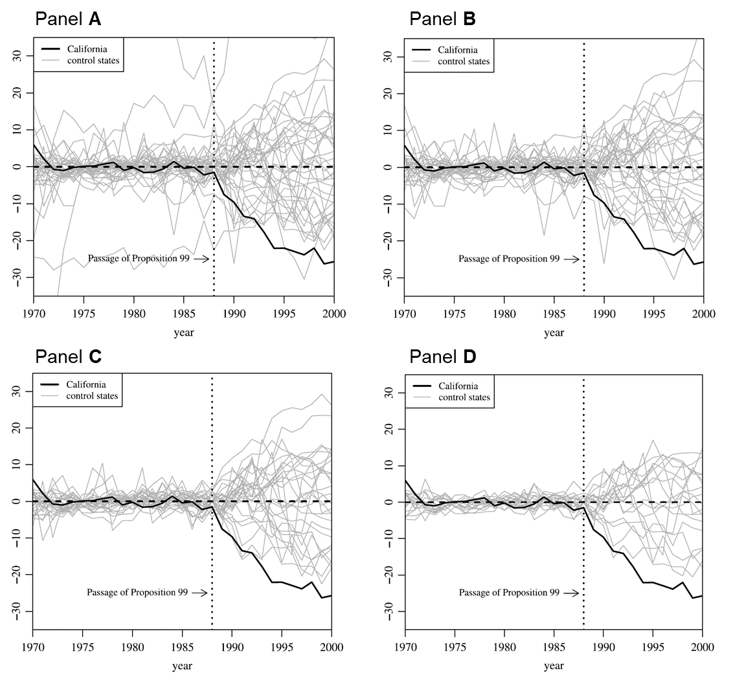
\includegraphics[scale=0.65]{F01}
	\caption{Region Exclusion Procedure of ADH}
	\label{F_01}
\end{figure}

One way to bypass the inefficient sample reduction procedure is to look at the distribution of the ratios of \ac{MSFE} and \ac{MSPE}. By scaling the post-treatment fit with the pre-treatment fit, regions with a poor fit are implicitly controlled for. In the tobacco control application, California is the region with the highest \ac{MSFE}-to-\ac{MSPE} ratio among all 39 regions which translates into a p-value of 2,6\% $\left(  \frac{1}{39} \right) $. 

\subsection{Simple Static Extension}
\textcolor{magenta}{\textbf{This is work in progress}}

\textcolor{magenta}{\textbf{to dos
		\begin{itemize}
			\item consistent notation
\end{itemize}}}

Consider a very simple framework for analyzing the causal effect of a treatment for unit $i = 0$ and two units in the control group $i = 1,2$. It is assumed that before the intervention at time period $t = T_0$ the units have a joint distribution of the form 
\[
\boldsymbol{y} = \begin{pmatrix} Y_1\\ Y_2\\ Y_3 \end{pmatrix} \sim \mathcal{N}(\boldsymbol{\mu},\boldsymbol{\Sigma})
\text{ before } T_0.
\] 
where $\boldsymbol{\mu} = \left(\mu_1, \mu_2, \mu_3  \right)^\prime$ and $\boldsymbol{\Sigma}$ is some positive definite covariance matrix with Choleski decomposition $\boldsymbol{\Sigma} = \boldsymbol{R}\boldsymbol{R}^\prime$ and $\boldsymbol{R}$ is an \textit{upper} triangular matrix. Assume that the intervention affects the mean of the first variable such that $\mathbb{E}(Y_0) = \mu_0 + \delta$ after the intervention, whereas the means of the other two variables remain unaffected. Accordingly, $\delta$ represents the treatment effect on $Y_0$. 

We are interested in deriving an optimal estimator for the counterfactual
\[
\widehat{Y}^{N}_{0} = \mathbb{E}(Y_0 | \delta = 0, Y_1, Y_2) \text{ after } T_0. 
\] 
Let $Q = R^{-1}$ and $q$ denotes the first row of $Q$, then
\[
q^\prime \boldsymbol{y} = q^\prime \boldsymbol{\mu} + \epsilon,
\] 
where $\epsilon \sim \mathcal{N}(0,1)$ with $\mathbb{E}(\epsilon | Y_!, Y_2) = 0.$ It follows that  
\begin{equation*}
	\begin{split}
		\widehat{Y}^{N}_{0} & = w_1 Y_1 + w_2 + Y_2 + \mu^* \\
		& = \mu_0 + w_1(Y_1 - \mu_1) + w_2(Y_2 - \mu_2),
	\end{split}
\end{equation*}
where $w_1 = -q_1/q_0$ and $w_2 = -q_2/q_0$ and $\mu^* = \mu_0 - w_1\mu_1 -  w_2\mu_2$. These results imply that there is no reason to impose the restrictions $w_1 \leq 0, w_2 \leq 0$ (positivity) and $w_1 + w_2 = 1$ (adding-up). Furthermore, the construction of \ac{SC} should include a constant term, as otherwise the \ac{SC} may have a different mean, See also \cite{doudchenko:2016} for a careful discussion of these restrictions.

For illustration assume that
\[
\boldsymbol{y} \sim \mathcal{N}\left( 
\begin{pmatrix} 1\\ 1\\ 1 \end{pmatrix}, 
\begin{pmatrix} 1 &0.1 &0.4\\0.1 &1 &0.5\\0.4 &0.5 &1 \end{pmatrix}\right) 
\] 
\textbf{Elaborate here once understood.} For this  example the optimal weights for the \ac{SC} result as $w_1 = -0.133$, $w_2 = 0.4667$ and $\mu^* = 1 - w_1 - w_2 = 0.667$. Note that $w_1$ is negative even all bivariate correlations between the panel units are positive. One may argue that this solution does not make much sense as from a economic perspective it is not clear what  it means that $Y_1$ enters the \ac{SC} with a negative sign. This demonstrates the trade-off between optimality in a statistical sense and the interpretability of the solution.

What happens if we impose the restrictions that all weights are positive and sum up to unity? In this case the restricted optimum yields the linear combination $\widetilde{Y}^{N}_{0} = 0.2 Y_1 + 0.8 Y_2$. The important difference lies in the variance of these estimates. For our example we obtain
\begin{equation*}
	\begin{split}
		& var(Y_0 - \widehat{Y}^{N}_{0}) = 0.827 \\
		& var(Y_0 - \widetilde{Y}^{N}_{0}) = 1.160		
	\end{split}
\end{equation*}
It is interesting to note that the variance of the restricted estimate is even larger than the unconditional variance of $Y_0$. This is possible as $(w_1, w_2) = (0,0)$ is not included in the restricted parameter space. 

It is not difficult to see that if $Y_0$ is not correlated with $Y_1$ and $Y_2$, then the optimal estimate boils down to $\widehat{Y}^{N}_{0} = \mu_0$ and therefore it does not make sense to involve a \ac{SC}. In microeconometric settings it is usually assumed that the individuals in the treatment group and individuals in th econtrol group are uncorrelated. In such cases we do not care about constructing a \ac{SC}. The crucial feature of \ac{SC} methods is the correlation between the units in the treatment and the control group. In macroeconomic applications however, the variables in the treatment and control group (e.g. \ac{GDP}) are typically correlated and it is therefore important to model the relationship between the variables. As the simple scenario with only two panel units in the donor pool is highly unrealistic in practice, we now move to the general static case with $k-1$ panel units.
\subsection{General Static Extension}
\textcolor{magenta}{\textbf{What must be clear by now
		\begin{itemize}
			\item Derive first analytical expressions for the case with $k$ donors before talking about regularization
\end{itemize}}}

In empirical practice it is often the case that the number of pre-intervention time periods $T_0 - 1$ is small and my even be smaller than the number of units in the donor pool, $k$.
\subsection{General Dynamic Extension}

\textcolor{magenta}{\textbf{What must be clear by now
		\begin{itemize}
			\item TBD
\end{itemize}}}
When modeling macroeconomic time series it is often assumed that the $(k+1)\times 1$ vector of time series $y_t = (Y_{0t}, ..., Y_{kt})^\prime$ can be represented by a \ac{VAR} model given by 